\documentclass{math}

\usepackage{tikz}

\title{Introduction to Computer Vision}
\author{Alvin Lin}
\date{August 2018 - December 2018}

\begin{document}

\maketitle

\section*{Face Detection}
The basic idea of face detection is to slide a window across the image and try
to evaluate a face model at every location. This technique must evaluate tens
of thousands of location/scale combinations. Since faces are relatively rare
in the space of an image, we should try to spend as little time as possible
on non-face windows for computational efficiency. \par
A megapixel image has \( 10^6 \) pixels and a comparable number of candidate
face locations. To avoid having a false positive in every image, our false
positive rate has to be less than \( 10^{-6} \).

\subsection*{Viola/Jones Face Detector}
The Viola/Jones face detector is a seminal approach to real time object
detection. While training is slow, detection is very fast. It involves
several key ideas:
\begin{itemize}
  \item \textbf{Integral images} for fast feature evaluation
  \item \textbf{Boosting} for feature selection
  \item \textbf{Attentional cascades} for fast rejection of non-face windows
\end{itemize}

\subsection*{Integral images}
An integral image contains, at each pixel \( (x,y) \), the sum of all pixel
values above and to the left of \( (x,y) \). This can be precomputed and used to
quickly compute the the sum of the pixel values within a rectangle. Suppose
\( A,B,C,D \) are the values of the integral image at the corners of an image.
\begin{center}
  \begin{tikzpicture}
    \draw (0,0) node[right]{A} -- (0,4) node[right]{B} --
      (-6,4) node[left]{C} -- (-6,0) node[left]{D} -- cycle;
  \end{tikzpicture}
\end{center}
The sum of the pixel values can be computed as \( A-B-C+D \). Only 3 addition
operations are required for any size of rectangle. This allows us to quickly
compute image features using rectangle filters. These rectangle filters usually
consist of a dark regions and a light regions to match corresponding
gradient changes in the target image.
\begin{center}
  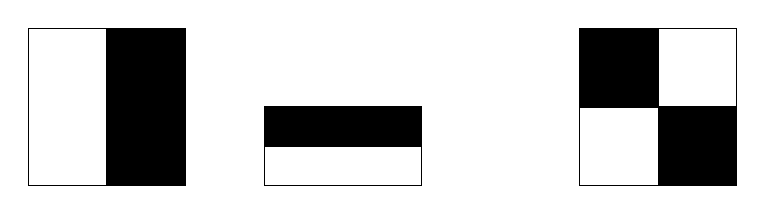
\begin{tikzpicture}
    \draw[draw=black] (0,0) rectangle ++(1,2);
    \draw[fill=black] (1,0) rectangle ++(1,2);
    \draw[draw=black] (3,0) rectangle ++(2,0.5);
    \draw[fill=black] (3,0.5) rectangle ++(2,0.5);
    \draw[draw=black] (7,0) rectangle ++(1,1);
    \draw[fill=black] (8,0) rectangle ++(1,1);
    \draw[draw=black] (8,1) rectangle ++(1,1);
    \draw[fill=black] (7,1) rectangle ++(1,1);
  \end{tikzpicture}
\end{center}

\subsection*{Feature Selection}
For a \( 24\times24 \) detection region, the number of possible rectangle
features as described above is \( \sim160000\). At test time, it is impractical
to evaluate the entire feature set, so we need to create a good classifier using
only a small subset of all such possible features.

\subsection*{Boosting}
Boosting is a classification scheme that works by combining weak learners into
a more accurate ensemble classifier. A weak learner only needs to perform better
than random classifications. Training consists of multiple boosting rounds where
a weak learner that does well on examples compared to previous learners is
selected. \par
Initially, each training example is weighted equally, but during each boosting
round we find the weak learner with the lowest weighted training error. We
raise the weights of the training examples misclassified by the current weak
learners. The final classifier is computed as a linear combination of all weak
learners where the weight of each learner is directly proportional to its
accuracy. Exact formulas for re-weighting and combining weak learners depend on
the particular boosting scheme. \par
Boosting integrates classification with feature selection and is empirically not
known to overfit. The complexity of training is linear in the number of training
examples. Boosting is also flexible in the choice of weak learners and boosting
schemes, fast, and easy to implement. However, it needs many training examples
and often doesn't work as well as a support vector machine (especially for
multi-class problems).

\subsubsection*{Boosting for Face Detection}
We define weak learners based on rectangular features and for each round of
boosting, we evaluate each rectangle filter on each example and select the
best filter/threshold combination to reweight the examples. This has a
complexity of \( O(mnk) \) with \( m \) rounds, \( n \) examples, and \( k \)
features.

\subsection*{Attentional Cascade}
We start with simple classifiers which reject many of the negative sub-windows
while detective almost all positive sub-windows. A positive response from the
first classifier triggers the evaluation of a second (more complex) classifier,
and so on. A negative outcome at any point leads to the immediate rejection of
the sub-window.
\begin{center}
  \begin{tikzpicture}
    \draw[->] node[left]{Image sub-window} (0,0) -- (1,0);
    \draw (2.5,0) circle (1.25cm) node[]{Classifier 1};
    \draw[->] (4,0) -- node[above]{T} (5,0);
    \draw[->] (2.5,-1.5) -- node[right]{F} (2.5,-2.5) node[below]{reject};
    \draw (6.5,0) circle (1.25cm) node[]{Classifier 2};
    \draw[->] (8,0) -- node[above]{T} (9,0) node[right]{face};
    \draw[->] (6.5,-1.5) -- node[right]{F} (6.5,-2.5) node[below]{reject};
  \end{tikzpicture}
\end{center}
These chain classifiers get progressively more complex and have lower false
positive rates. The detection rate and the false positive rate of the cascade
are found by multiplying the respective rates of the indvidual rates of the
individual stages. A detection rate of 0.9 and a false positive rate on the
order of \( 10^{-6} \) can be achieved by a 10-stage cascade if each stage
has a detecton rate of 0.99 and a false positive rate of about 0.3 since
\( 0.99^10 \approx 0.9 \) and \( 0.3^10 \approx 6\times10^{-6} \).

\subsubsection*{Training the Cascade}
\begin{itemize}
  \item Set the target detection and false positive rates for each stage.
  \item Keep adding features to the current stage until its target rates have
    been met. We may need to lower the AdaBoost threshold to maximize detection.
    This should be tested on a validation set.
  \item If the overall false positive rate is not low enough, then add another
    stage.
  \item Use false positives from the current stage as the negative training
    examples for the next stage.
\end{itemize}

\begin{center}
  You can find all my notes at \url{http://omgimanerd.tech/notes}. If you have
  any questions, comments, or concerns, please contact me at
  alvin@omgimanerd.tech
\end{center}

\end{document}
